%%%%%%%%%%%%%%%%%%%%%%%%%%%%%%%%%%%%%%%%%%%%%%%%%%%%%%%%%%%%%%%%%%%%%%%%%
%
% This file defines the style for your homebook
% You don't need to edit it any more, if not to 
% change the authors name:
%
% Search below for the keyword:   GROUP
% insert your group number
%
% Search below for the keyword:   AUTHORS
% insert the name of the authors
%
%%%%%%
% Now to update the dexcription  of your work you will 
% use the file ``master.tex'' in the current directory
% following the instructions in it 
%
%%%%%% 
%%%%%%  
%%%%%%
% If you want to compile your document you have TWO ways
% depending on the fact that 
% 	1) you have inserted only postcript images in your tex file 
%		---> then go to MODE 1
%	2) you have inserted other kind of images (jpg..) in your tec file
%		---> then go to MODE 2
%
% MODE 1 
%simple type:
% 	latex homebook.tex
%
% If the compilation runs succesfully and you want to see the results type:
% 	xdvi homebook.dvi &
% and use the menus to go through the document
%
% If you want to create a pdf type:
% 	dvipdfm homebook.dvi
%
% a homebook.pdf file is created
% you can see it using the command:
% 	acroread homebook.pdf &
%
%
% MODE 2
% simple type:
%	pdflatex homebook.tex
%
% If the compilation runs succesfully you directly have the pdf file
% and you can see it using the command:
%       acroread homebook.pdf &
%
% 
%%%%%%%%%%%%%%%%%%%%%%%%%%%%%%%%%%%%%%%%%%%%%%%%%%%%%%%%%%%%%%%%%%%%%%%%%%
\documentclass[10pt,  english, makeidx, a4paper, titlepage, oneside]{book}
\usepackage{babel}
\usepackage{fancyhdr}
\usepackage{makeidx}
\usepackage{titlesec}
\usepackage{listings} 
\usepackage{siunitx}
\usepackage{float}
\usepackage{mathtools}



\newenvironment{listato}{\footnotesize}
                        {\normalsize }


%\pagestyle{empty}

\textwidth 15.5cm
\textheight 23cm
\topmargin -1cm
\oddsidemargin -0.5cm
\linespread{1.1}

\pagestyle{fancy}
\lhead{}
\chead{Integrated Systems Architecture}
\lfoot{}
\cfoot{}
\rfoot{}
\rhead{\thepage}

\usepackage{graphicx}
\usepackage{amsmath}
\usepackage{amsfonts}
\usepackage{amsthm}
\usepackage{amssymb}
%\oddsidemargin -1.1cm

\titleformat{\chapter}[display]
{\normalfont\Large\filcenter\sffamily}
{\titlerule[0.5pt]%
\vspace{1pt}
\titlerule
\vspace{1pc}
\LARGE\MakeUppercase{\chaptertitlename} \thechapter
}
{1pc}
{\titlerule
\vspace{1pc}
\Huge}

\newcommand{\SubSubSection}[1]{\subsubsection{\bf Exercise   ~#1}}

\newcommand{\homework}[1]{\subsubsection{\bf Homework   ~#1}}

\newcommand{\Solution}{\subsubsection{\bf Solution}}




\makeindex
\begin{document}
\frontmatter
\begin{titlepage}
\vspace{2cm}
\centerline{
\includegraphics[width=2cm]{./logopoli}}  
\centerline{\LARGE Politecnico di Torino}
\bigskip
\centerline{\Large III Facolt\`a di Ingegneria}
\vspace{4cm}
\centerline{\Huge\sf Digital Arithmetic and Logic Sythesis}
\vspace{2cm}
\centerline{\LARGE Master degree in Electriconic Engineering}
\bigskip
\centerline{\LARGE Integrated Systems Architectures}
\vspace{4.4cm}
%%%%%%%%%%%%%%%%%%%%%%%%%%%%%%%%%%%%%%%%%%%%%%%%%%%%%%%
% GROUP
% Change the name of your group below
%
\centerline{\Large Authors: Group 34}
\bigskip
\centerline{\Large github repository link :}
\bigskip
\centerline{\Large https://github.com/alessionaclerio22/Integrated-Systems-Architecture-Labs}
\vspace{2cm}
%
%%%%%%%%%%%%%%%%%%%%%%%%%%%%%%%%%%%%%%%%%%%%%%%%%%%%%%%
% AUTHORS
% Change the name of the Group participants here
%
\centerline{Simone Di Blasi, Stefano Floridia, Alessio Naclerio}
%
%%%%%%%%%%%%%%%%%%%%%%%%%%%%%%%%%%%%%%%%%%%%%%%%%%%%%%

\end{titlepage}

\tableofcontents

%%%%%%%%%%%%%%%%%%%%%%%%%%%
% 
\mainmatter
\lstset{language=VHDL}

%%%%%%%%%%%%%%%%%%%%%%%%%%%%%%%%%%%%%
%%%%%%%%%%%%%%%%%%%%%%%%%%%%%%%%%%%%%
%%    
%% HERE IS THE MAIN INCLUSION
%%
\chapter{Floating Point Multiplier Synthesis}
\label{chap1}

The main goal of this laboratory is to exploit Synopsys Design Compiler to compare the results obtained by different synthesis performed on the floating point multiplier. This is a pipelined component that is included in the "Floating Point Adder and Multiplier" project, which has been downloaded from Portale della Didattica.

\section{Multiplier Simulation}

First of all, a testbench has been created in order to test the correctness of the multiplier. Hence, the work environment has been organized in three main folders, $src$ containing all the source $.vhd$ files, $tb$ with all testbench-related files and $sim$ for the simulation with $ModelSim$. Then, $sim$ has been subdivided in different subfolders. In order to perform the simulation, $clk\_gen.vhd$, $data\_maker.vhd$ and $tb\_fpmul.v"$ in folder $tb$ have been used. They respectively generate a $10\si{\nano\second}$ clock signal, feed the multiplier with the values provided in $fp\_samples.hex$ and connect the DUT to the testbench. Then, in subfolder $sim\_init$, the script $compile.sh$ has been run in order to compile all needed files. At last, the simulation has been carried out using $ModelSim$ and a $pdf$ file has been generated with the resulting waveforms. The results have been compared with the one in $fp\_prod.hex$ in order to check their correctness.
\newline
\newline
\noindent The same flow has been adopted for the next point of the assignment, where it is asked to add a register to the inputs of the multiplier. After properly modifying $fpmul\_pipeline.vhd$, the previous steps have been followed changing the simulation folder to $sim\_reg$. At last, a $pdf$ file has been created showing the waveforms and the obtained results have been checked against the ones contained in $fp\_prod.hex$.

\section{Synthesis}

Using the floating point pipelined multiplier with the additional registers at the inputs, various synthesis have been carried out. As a matter of fact, the aim of this part of the laboratory is to force Synopsys Design Compiler to use a specific architecture for the behavioural multiplication in $fpmul\_stage2\_struct.vhd$ and compare the different results in terms of maximum frequency and area.
In order to do this, a folder called $syn$ has been created. As requested by the assignment, three synthesis have been performed respectively asking to:

\begin{itemize}
\item force Synopsys Design Compiler to flatten the hierarchy;
\item force Synopsys Design Compiler to flatten the hierarchy and implement the multiplier in Stage2 as a CSA multiplier;
\item force Synopsys Design Compiler to flatten the hierarchy and implement the multiplier in Stage2 as a PPARCH multiplier.
\end{itemize}

\noindent In order to fulfill these requirements, the subfolders $syn\_first$, $syn\_CSA$ and $syn\_PPARCH$ have been created inside $syn$, each related to the correspondent synthesis. Three similar $tcl$ scripts have been exploited to speed up the Synopsys Design Compiler flow, $syn\_first.tcl$, $syn\_CSA.tcl$ and $syn\_PPARCH.tcl$. They all contain the same commands in order to set up the synthesis and to flatten the hierarchy ($ungroup  -all -unflatten$). However, $syn_CSA.tcl$ and $syn\_PPARCH.tcl$ force an implementation with the command $set\_implementation$, while $syn\_first.tcl$ does not.
In order to obtain the maximum frequency, an iterative approach has been adopted setting the clock to $0\si{\nano\second}$ as first step and then adding the retrieved slack until $report\_timing$ gives a null slack. Three files have been generated for each synthesis containing the outcome of the commands $report\_resources$, $report\_area$ and $report\_timing$. The obtained values have been summarized in Table.


\section{Fine-grain Pipelining and Optimization}

In this part of the laboratory, it is asked to modify the Stage2 structure by adding a register at the output of the significand multliplier and all the required ones to preserve the right pipeline behaviour. In order to do this, a file called $fpmul\_stage2\_struct\_modified.vhd$ has been created. It contains the Stage2 architecture modified as requested by the assignment. It has been simulated using the same testbench files mentioned before, changing the simulation environment to folder $sim\_modified$. In this folder, the script $compile.sh$ has been used to compile the needed files, this time substituting $fpmul\_stage2\_struct.vhd$ with $fpmul\_stage2\_struct\_modified.vhd$. A $pdf$ file has been generated to check the correctness of the waveforms and the results have been compared to the ones in $fp\_prod.hex$.
\newline
\newline
\noindent Using the modified structure for the floating point multiplier, two additional synthesis have been carried out. The $syn$ subfolders $syn\_modified$ and $syn\_modified\_ultra$ have been used for this purpose. The main goal of this part is to investigate the results obtained by the commands $optimize\_registers$ after $compile$ and $compile\_ultra$ instead of the combination of the previous two. The synthesis have been perfomed using $tcl$ scripts issuing the above mentioned operations. An iterative approach has been adopted in order to obtain the maximum frequency, as described in the previous section. Moreover, $report\_area$ and $report\_timing$ have been generated in each subfolder. The results concerning maximum frequency and area are summarized in Table.




\chapter{Modified Booth Encoding Multiplier}
\label{chap2}


\section{MBE Multiplier Design}
In order to complete the set of comparisons among different multiplier's implementations,
a modified-Booth-encoding multiplier for unsigned data has been designed. In the folder $MBE\_multiplier$, three subfolders
have been created, $src$, $tb$ and $sim$.
In order to follow the specifications given by the assignment, partial products have been
generated without using any adders or subtracters, the adder plane has been implemented
relying on a Dadda tree and sign extension bits have been simplified as proposed in the
file $sign\_extension\_booth\_multiplier\_Stanford.pdf$. Once the simulation has been carried
out to check its correctness, the MBE multiplier has been exploited in the Stage2 of the
floating point multiplier, instead of the behavioural one "$*$".

\begin{figure}[H]
	\centering
	\includegraphics[width=\textwidth , height=10cm]{img/MBE_Mult.png} 
	\caption{Modified Booth encoding multiplier block diagram}
	\label{Modified Booth encoding multiplier block diagram} 
\end{figure}

As depicted in figure, the main blocks used in this design are:

\begin{itemize}
 
\item \emph{MBE\_recoder}: based on the input triplet coming from the operand $b$, it provides the correct partial product 
at the output, according to the table shown in Figure 2.2;

\item \emph{A\_gen}: it generates the values that will be fed to the $MBE\_recoder$. It takes
$a$ on 32 bits as input and it provides four 33-bit outputs, $a$ (setting '0' as MSB), $2a$,
1's complement $a$ and 1's complement $2a$;

\item \emph{Sign\_Ext}: it selects the value for $S$ as indicated in the file
$sign\_extension\_booth\_multiplier\_Stanford.pdf$. If the partial product is negative, $S$ will be 
equal to '1' in order to add 1 to the toggled version of $a$ or $2a$ and generate the correct
2's complement value. If the partial product is positive, $S$ will be '0' in order to clear
the sign extension bits;

\item \emph{Dadda\_Tree}: it performs the addition on the 17 sign-extended partial products as
stated by the Dadda algorithm. Starting from the initial "Staircase" form, partial products have been reorganized in a "V-shape" structure, where each column contains equally-weighted bits. Both forms are depicted respectively in Figure 2.3 and Figure 2.4. Also $S$
bits have been properly assigned. Since 17 partial products are present, 6 reduction operations have to be performed before having the final 2 operands on which a behavioural
addition has been perfomed. At each level, the minimum number of HA and FA have been assigned
in order to reach the next level's maximum heigth. As described by comments in file "Dadda\_Tree.vhd", a three-dimensional array has been exploited to have 7 different "V-shape" matrices, each corresponding to a reduction level. For each of this levels, the Dadda Algorithm has been applied, until reaching the final two partial products;

\end{itemize}


\begin{figure}[H]
	\centering
	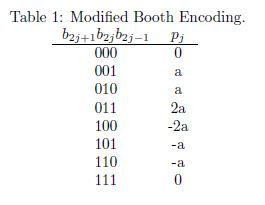
\includegraphics[width=8cm, height=6cm]{img/MBE.jpeg} 
	\caption{Recoding Table}
	\label{Recoding Table} 
\end{figure}

\begin{figure}[H]
	\centering
	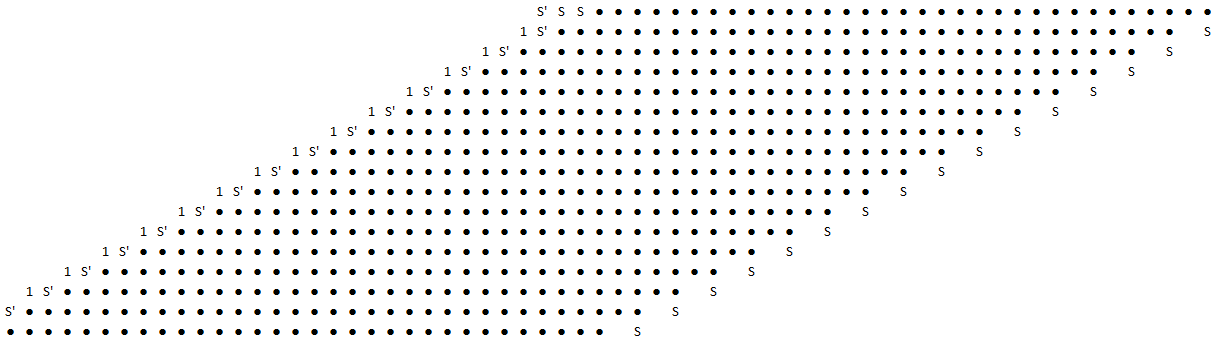
\includegraphics[width=\textwidth , height=10cm]{img/staircase.png} 
	\caption{Staircase partial products matrix}
	\label{Staircase partial products matrix} 
\end{figure}

\begin{figure}[H]
	\centering
	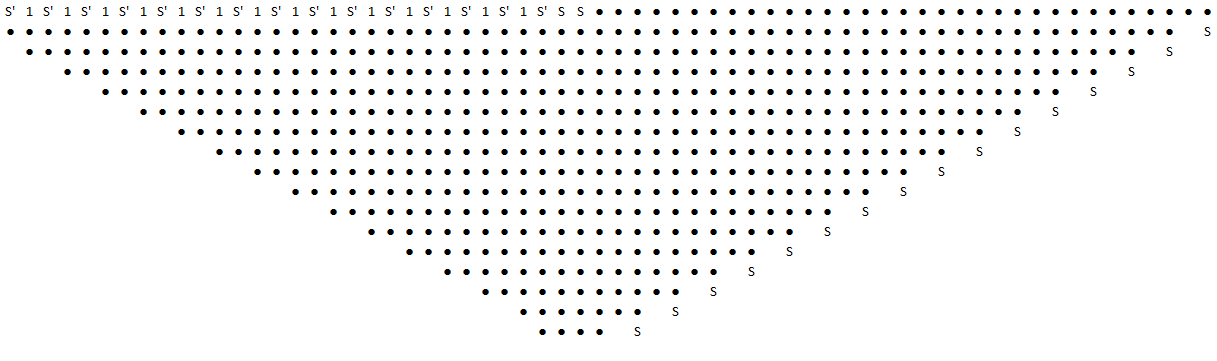
\includegraphics[width=18 cm , height=10cm]{img/vshape.png} 
	\caption{V-shape partial products matrix}
	\label{V-shape partial products matrix} 
\end{figure}

All these components have been used in the top entity "Dadda\_Multiplier", connected as depicted in
figure. As mentioned before, a behavioural adder "$+$" has been exploited in order to add the final
reduction level partial products.

\section{MBE Multiplier Simulation}

A simulation of the designed multiplier has been carried out using $tb\_Dadda\_Mul.vhd$ in subfolder $tb$. 
This testbench exploits a 32-bits LFSR generating the multiplier's inputs. The same values are given to a behavioural
unsigned multiplier in order to check the correctness. If the two outputs are equal, a "check signal" is equal to one.
The simulationn has been performed in the subfolder $sim$ using the script $compile.sh$ to compile the needed files.
It has been run for in order to verify the correct behaviour of the component and a $pdf$ file containing the resulting
waveforms has been saved.
\newline
\newline
Then, the a new file called $fpmul\_stage2\_struct\_MBE.vhd$ has been created starting from $fpmul\_stage2\_struct.vhd$
by replacing the behavioural multiplier with the MBE one. A new subfolder named $sim_MBE$ has been created in folder $sim$ and
the simulation has been run with the help of $compile.sh$. The resulting values have been checked and a $pdf$ file has been generated
with the obtained waveforms.

\section{MBE Multiplier Synthesis and Final Comparison}

Once the correctness has been verified, a subfolder called $syn\_MBE$ has been created in $syn$ and set as work environment for the
synthesis. It has been perfomed using a $tcl$ script and an iterative approach has been adopted in order to obtain the maximum frequency, as described in the previous paragraph. Moreover, an area report and a timing report have been produced in order to check the results concerning maximum frequency and area, which are summarized in Table along with all the others.



\begin{center}
    \begin{tabular}{ |c|c|c|c| } 
        \hline
            Name & $t_{min}$[$\si{\nano\second}$] & $f_{max}$[$\si{\mega\hertz}$] & area[$\si{\micro\meter}^{2}$]\\
            \hline
            syn\_first & 1.56 & 641.025641 & 4047.721967\\
            \hline
            syn\_CSA & 4.28 & 233.644859 & 3712.828004\\
            \hline
            syn\_PPARCH & 1.56 & 641.025641 & 4097.197964\\
            \hline
            syn\_modified & 0.87 & 1149.42528 & 5572.433932\\
            \hline
            syn\_modified\_ultra & 1.50 & 666.666666 & 4207.321944\\
            \hline
            syn\_MBE & 4.10 & 243.902439 & 6905.625925\\
        	\hline
    \end{tabular}
    \begin{center}
    	Table 1: Comparisons Table.
    \end{center}
\end{center}


\subsection{Final Overall Comparisons}

Regarding the maximum frequency, the best result has been obtained with the synthesis using the command $optimize\_registers$, which applies a proper retiming to the design. The same clock has been retrieved for the first synthesis and the one forcing a PPARCH implementation. As a matter of fact, looking at the files generated by $report\_resources$, the same multiplier implementation is used in both of them. The worst one in terms of timing is the CSA one, with $4.28\si{\nano\second}$.
As shown in figure, the best one in terms of area occupation is the CSA, while the worst is the MBE implementation. As before, the first synthesis and the PPARCH one are very similar, with the latter a little bit greater than the first. As regards the $compile\_ultra$ results, it has a lower area occupation than the $optimize\_registers$ version. However, it also shows a greater clock period leading to a lower maximum frequency.

\appendix
\chapter{Documents}
\label{appendix1}

The folders organization are the following:\\
\begin{itemize}
    \item MBE\_Multiplier
    \begin{itemize}
        \item sim (Simulation files)
         \begin{itemize}
            \item compile 
            \item sim\_MBE.pdf
            \item sim\_MBE.ps
        \end{itemize}
        \item src (VHD files)
         \begin{itemize}
            \item A\_gen
            \item Dadda\_Multiplier
            \item Dadda\_Tree
            \item FA
            \item HA
            \item MBE\_recoder
            \item Sign\_Ext
            \item types
        \end{itemize}
        \item tb (Test-bench files)
         \begin{itemize}
            \item tb\_Dadda\_Mul 
        \end{itemize}
    \end{itemize}
    \item sim (Simulation Files)
    \begin{itemize}
        \item sim\_init
         \begin{itemize}
            \item compile
            \item fp\_prod.hex
            \item fp\_samples.hex
            \item sim\_first.pdf
            \item sim\_first.ps
        \end{itemize}
        \item sim\_MBE
         \begin{itemize}
            \item compile
            \item fp\_prod.hex
            \item fp\_samples.hex
            \item sim\_MBE.pdf
            \item sim\_MBE.ps
        \end{itemize}
        \item sim\_modified
         \begin{itemize}
            \item compile
            \item fp\_prod.hex
            \item fp\_samples.hex
            \item sim\_modified.pdf
            \item sim\_modified.ps
        \end{itemize}
        \item sim\_reg
         \begin{itemize}
            \item compile
            \item fp\_prod.hex
            \item fp\_samples.hex
            \item sim\_reg.pdf
            \item sim\_reg.ps
        \end{itemize}
    \end{itemize}
    \item src (VHD files)
        \begin{itemize}
            \item fpmul\_pipeline
            \item fpmul\_pipeline\_first
            \item fpmul\_single\_cycle
            \item fpmul\_stage1\_struct
            \item fpmul\_stage2\_struct
            \item fpmul\_stage2\_struct\_MBE
            \item fpmul\_stage2\_struct\_modified
            \item fpmul\_stage3\_struct
            \item fpmul\_stage4\_struct
            \item fpnormalize\_fpnormalize
            \item fpround\_fpround
            \item packfp\_packfp
            \item unpackfp\_unpackfp
        \end{itemize}
    \item syn (Synthesis Files)
    \begin{itemize}
        \item syn\_csa
         \begin{itemize}
            \item report\_area\_CSA
            \item report\_timing\_CSA
            \item report\_res\_CSA
            \item syn\_CSA
        \end{itemize}
        \item syn\_first
         \begin{itemize}
            \item report\_area\_first
            \item report\_timing\_first
            \item syn\_first
        \end{itemize}
        \item syn\_MBE
         \begin{itemize}
            \item report\_area\_MBE
            \item report\_timing\_MBE
            \item report\_res\_MBE
            \item syn\_MBE
        \end{itemize}
        \item syn\_modified
         \begin{itemize}
            \item report\_area\_modified
            \item report\_timing\_modified
            \item report\_res\_modified
            \item syn\_modified
        \end{itemize}
        \item syn\_modified\_ultra
         \begin{itemize}
            \item report\_area\_modified\_ultra
            \item report\_timing\_modified\_ultra
            \item report\_res\_modified\_ultra
            \item syn\_modified\_ultra
        \end{itemize}
        \item syn\_PPARCH
         \begin{itemize}
            \item report\_area\_PPARCH
            \item report\_timing\_PPARCH
            \item report\_res\_PPARCH
            \item syn\_modified\_PPARCH
        \end{itemize}
    \end{itemize}
    \item tb (Test-bench files)
         \begin{itemize}
            \item clk\_gen
            \item data\_maker
            \item tb\_fpmul
        \end{itemize}    
\end{itemize}
%%
%% NOW READ THE FILE master.tex  
\end{document}

